\documentclass{article}[11pt]
%Required: You must have these
\usepackage{graphicx}
\usepackage{tabularx}
\usepackage{natbib}

\usepackage{array}
\usepackage{amsmath}
%\usepackage[backend=bibtex]{biblatex}
\setkeys{Gin}{width=0.8\textwidth}
%\setlength{\captionmargin}{30pt}
\setlength{\abovecaptionskip}{10pt}
\setlength{\belowcaptionskip}{10pt}
\topmargin -1.5cm 
\oddsidemargin -0.04cm 
\evensidemargin -0.04cm 
\textwidth 16.59cm
\textheight 23.94cm 
\parskip 7.2pt 
\renewcommand{\baselinestretch}{1.2} 	
\parindent 0pt


\bibliographystyle{..//refs/styles/besjournals.bst}
\renewcommand{\thetable}{S\arabic{table}}
\renewcommand{\thefigure}{S\arabic{figure}}
%\usepackage{xr}
%\usepackage{hyperref}
\usepackage{xr-hyper}
\usepackage{hyperref}
\externaldocument{outline}


\title{Supporting Information for: Flower-leaf phenological sequences in the American Plums (\textit{Prunus} sect. \textit{Prunocerasus}) reflect adaption to aridity}

\usepackage{Sweave}
\begin{document}
\input{suppliment-concordance}
\maketitle

\section*{Figures} 
\begin{figure}[h!]
    \centering
 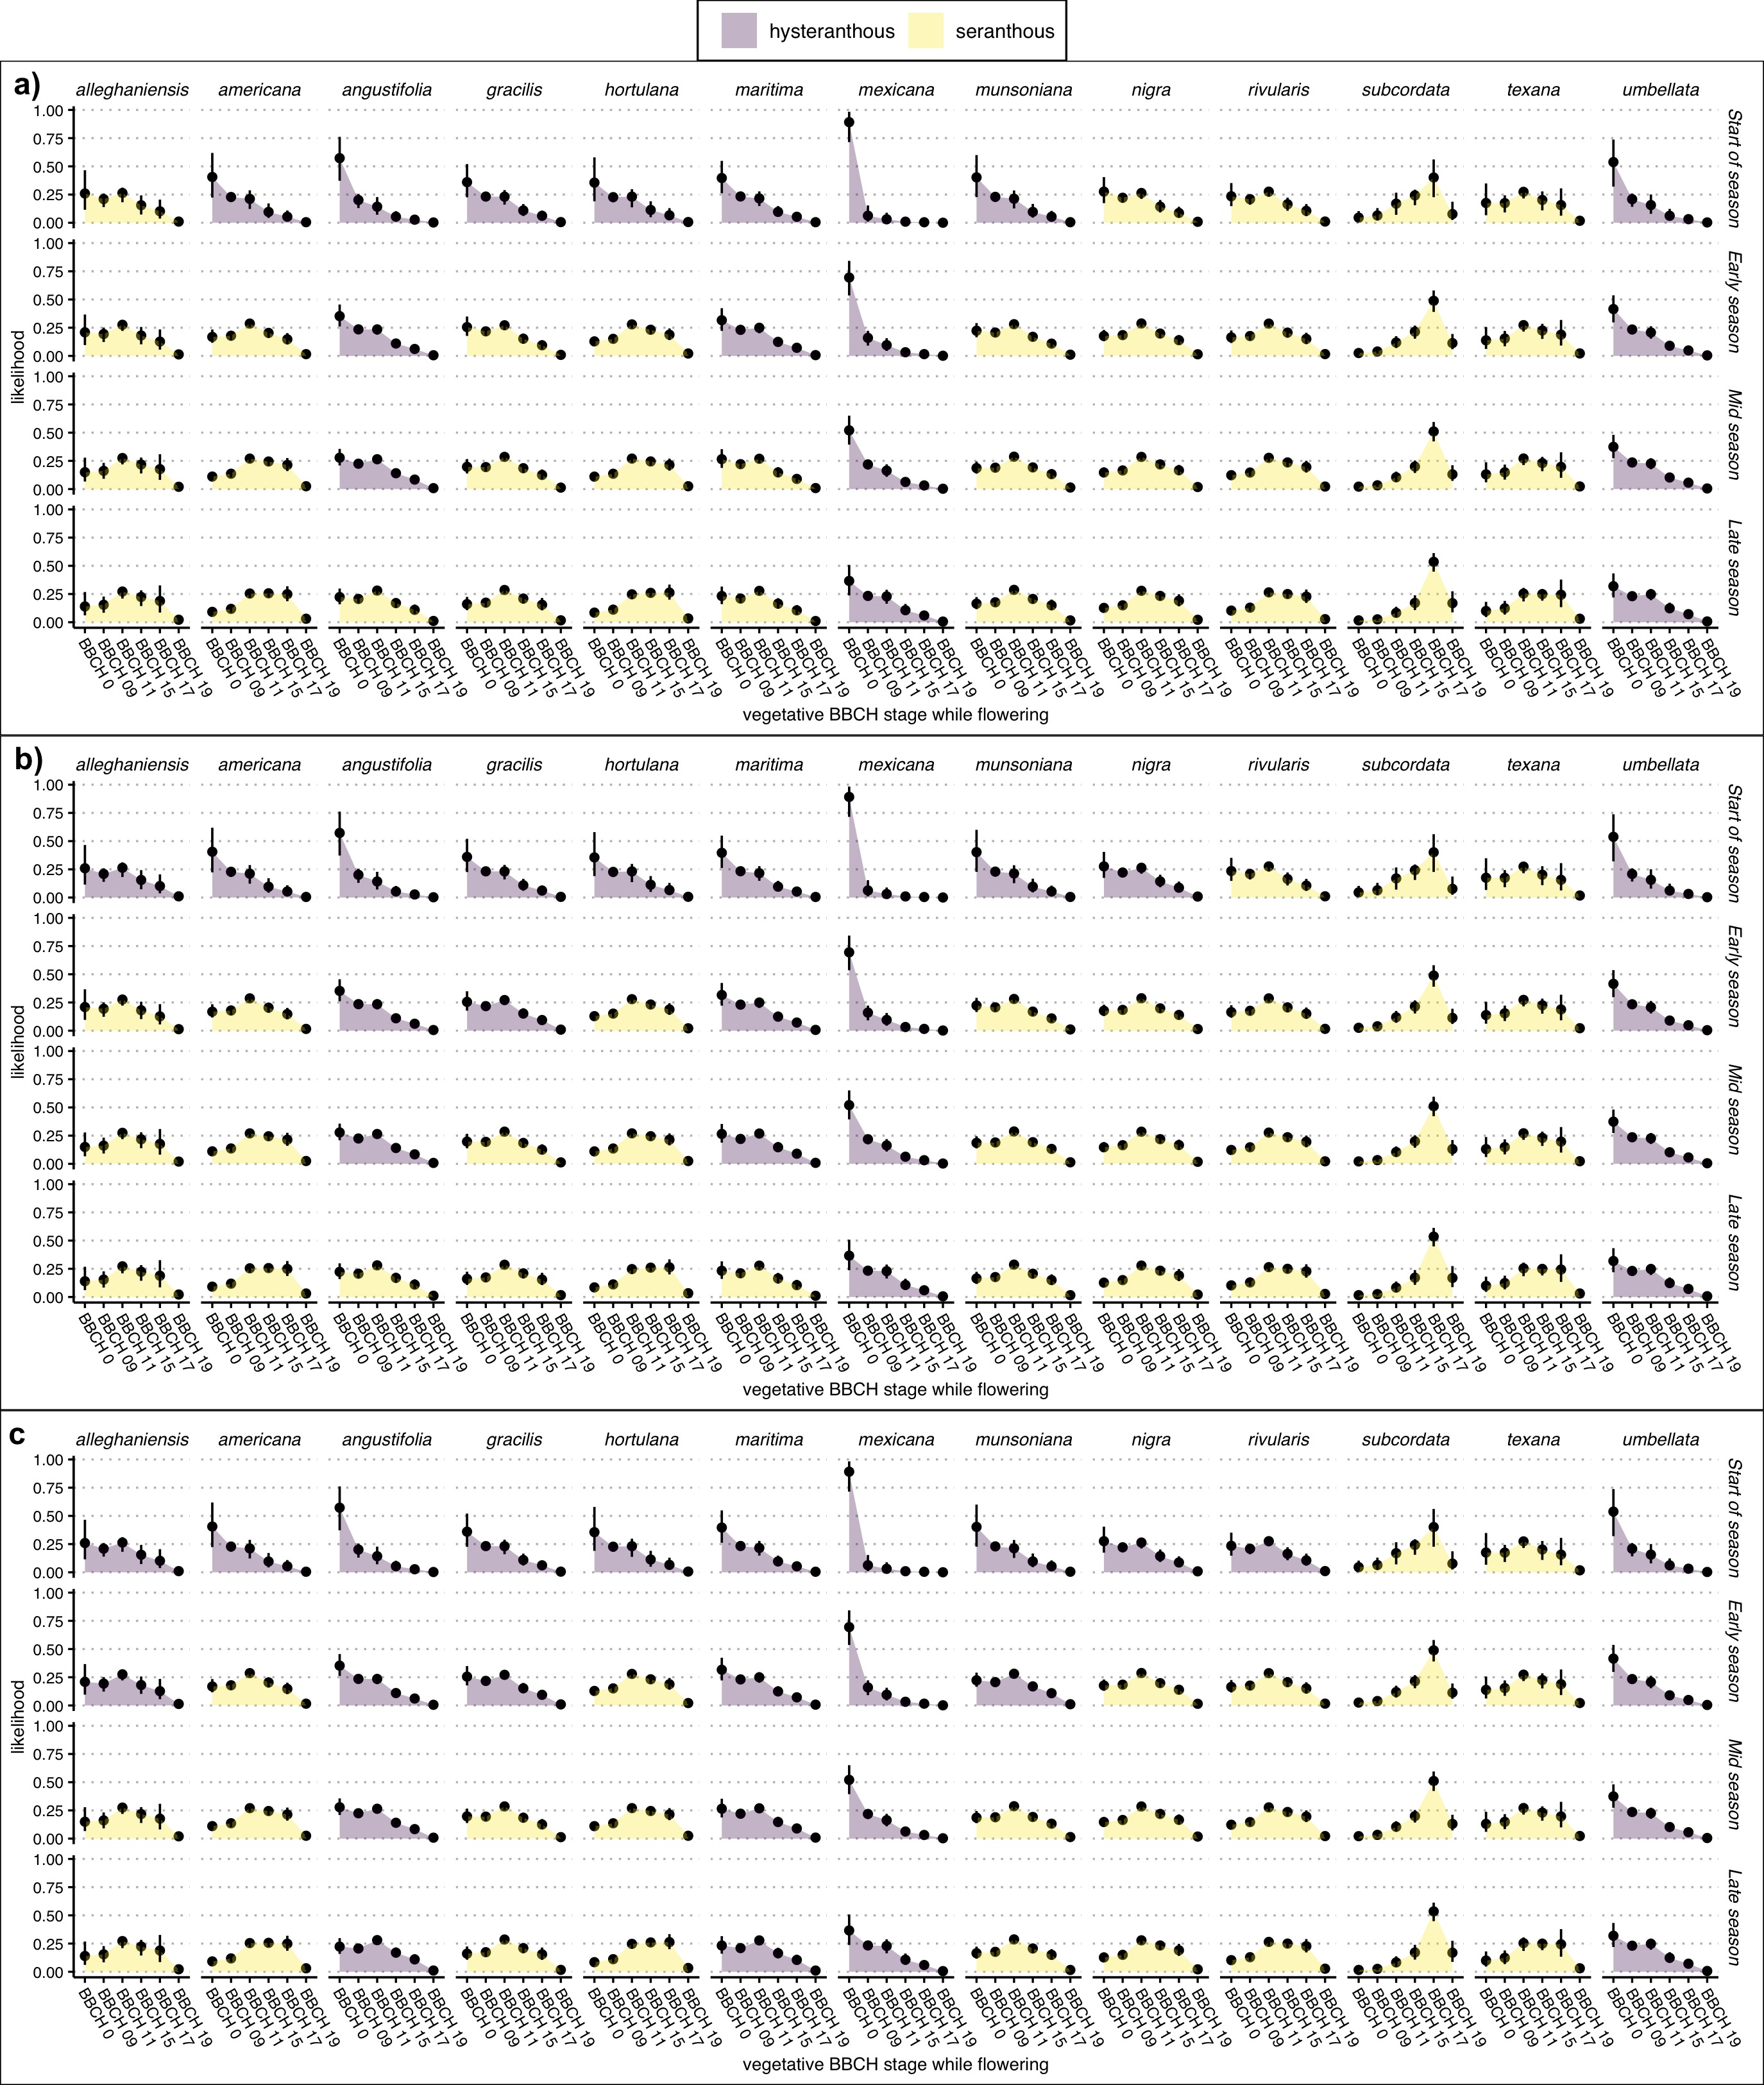
\includegraphics[width=\textwidth]{..//..//Plots/ord_quants_phylo.jpeg}
    \caption{Say better: The likihood a species will be at a given vegetative bbch stage during flowering at 4 different time point across their flowering season. Colors indicate whethere a species what classified as hysteranthous or not. a) b) and c) are the products of the different schemes.}
    \label{fig:plums}
\end{figure}

\section*{Tables}
\begin{table}[ht]
\centering
\begin{tabular}[width=.8\textwidth]{|lllrrrrrr|}
  \hline
  mod\_variable & classification & Hystanthous\_if & Estimate & Error & Q2.5 & Q25 & Q75 & Q97.5 \\ 
  \hline
 mean pdsi & main & 50\% fl. likelihood with BBCH 0 \& 09 & -0.03 & 0.02 & -0.08 & -0.05 & -0.02 & 0.01 \\ 
   mean pdsi & alternate 1 & 25\% fl. likelihood with BBCH 0 & -0.03 & 0.03 & -0.08 & -0.04 & -0.01 & 0.02 \\ 
  mean pdsi & alternate 2 & 40\% fl. likelihood with BBCH 0 \& 09 & -0.03 & 0.03 & -0.08 & -0.04 & -0.01 & 0.02 \\ 
  \hline
   petal length & main & 50\% fl. likelihood  with BBCH 0 \& 09 & -0.21 & 0.28 & -0.74 & -0.38 & -0.04 & 0.34 \\ 
  petal length & alternate 1 & 25\% fl. likelihood with BBCH 0 & -0.16 & 0.29 & -0.74 & -0.34 & 0.02 & 0.43 \\ 
  petal length & alternate 2 & 40\% fl. likelihood with BBCH 0 \& 09 & -0.26 & 0.27 & -0.80 & -0.43 & -0.09 & 0.30 \\ 
 \hline
 fruit diameter & main & 50\% fl. likelihood  with BBCH 0 \& 09 & -1.40 & 0.90 & -3.17 & -1.97 & -0.82 & 0.40 \\ 
  fruit diameter & alternate 1 & 25\% fl. likelihood with BBCH 0 & -1.77 & 0.93 & -3.59 & -2.35 & -1.20 & 0.09 \\ 
  fruit diameter & alternate 2 & 40\% fl. likelihood with BBCH 0 \& 09 & -1.83 & 0.89 & -3.60 & -2.36 & -1.28 & -0.09 \\ 
   \hline
\end{tabular}
\caption{Estimates of the relation ship betwen hysteranthy index and traits for our main model and alternative models based on different classification schemes of the hysteranthy index. All models give similar answers so yay.}
\label{tab:modput}
\end{table}


\end{document}
